\chapter{Configuração da Análise}
\label{ch:ferramentas}

\section{Setup Inicial em Debian}

Utilizamos o Debian 64 bits como sistema operacional. Segundo o próprio autor \cite{spi}, o sistema proporciona um bom funcionamento com pacotes básicos do sistema. Além disso, o Debian permite um setup padrão rápido para o trabalho com um script bash, podendo ser reproduzido em outras máquinas de forma prática.

Inicialmente precisamos instalar o Virtual Box \cite{oracle_vb}, GNS3 \cite{gns3_install} e Wireshark \cite{linoxide} para realizar os devidos testes.
\begin{lstlisting}[language=bash]

  # Adicao de Repositorios e Arquivos
  sudo add-apt-repository ppa:gns3/ppa
  
    deb http://download.virtualbox.org/virtualbox/debian xenial contrib
  sudo apt-key add oracle_vbox_2016.asc
  sudo apt-key add oracle_vbox.asc
  wget -q https://www.virtualbox.org/download/oracle_vbox_2016.asc -O- | sudo apt-key add -
  wget -q https://www.virtualbox.org/download/oracle_vbox.asc -O- | sudo apt-key add -
  
  # Atualizacao
  sudo apt-get update
  
  # Instalacao do Virtual Box
  sudo apt-get install virtualbox-5.1
  
  # Instalacao do Wireshark
  sudo apt-get install wireshark
  
  # Instalacao do GNS3
  sudo apt-get update
  sudo apt-get install gns3-gui

  
\end{lstlisting}

Com estes comandos, o nosso sistema Debian está pronto para iniciar as devidas configurações para a análise.

Vale ressaltar que é possível realizar os mesmos testes em outros sistemas (Outras distribuições linux, Windows e Mac), sendo somente de escolha por comodidade e conhecimento de todos os integrantes do projeto.
% mudanças do Christopher:
% distros -> distribuições
% ambos os integrantes -> todos os integrantes

\section{Configuração do Virtual Box}

Criamos duas máquinas virtuais, ambas com sistema Debian 64bits. As configurações utilizadas foram as seguintes:
   
\begin{table}[H]
\centering
%\caption{Tabela de Configurações das Máquinas Virtuais}
\label{my-label}
\begin{tabular}{|l|l|l|}
\hline
Características   & Servidor                        & Cliente                          \\ \hline
HD                & 8GB                             & 8GB                              \\ \hline
RAM               & 1024MB                          & 512MB                            \\ \hline
VRAM              & 16MB                            & 128MB                            \\ \hline
ADAPTADOR DE REDE & PRO/1000 MT Server (GNS3) & PRO/1000 MT Desktop (GNS3) \\ \hline
\end{tabular}
\caption{Tabela de Configurações das Máquinas Virtuais}
\end{table}

\section{GNS3}

Para este projeto, utilizamos um servidor local do GNS3, utilizando IOs da CISCO \cite{ciscoios}.

Para adicionar uma IOs, é necessário ir em Preferências -> IOs Routing, e selecionar a devida imagem do sistema a carregar.
% será necessário -> é necessário


\begin{figure}[H]
\centering
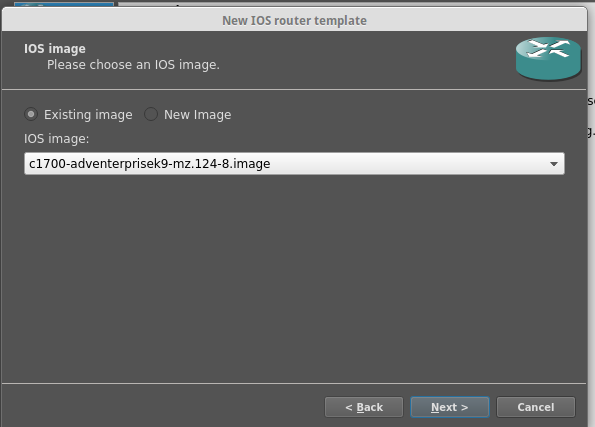
\includegraphics[width=10cm]{003.png}
\caption{Seleção da IOS}
\label{Rotulo}
\end{figure}

O Roteador utilizado neste \textit{setup} para a análise será o C1700, que já possui entrada para duas interfaces, que será o básico para conectar as duas máquinas virtuais já configuradas no Virtual Box.
%análise, será -> análise será
%já que -> que já (acho que fica melhor, mas sei lá)

Outra configuração necessária é a adição dos Hosts do Virtual Box. Para isso, deve-se abrir a aba de Hosts, e selecionar "New Appliance Template", selecionando em seguida "Add a VirtualBox Virtual Machine", e selecionando as duas máquinas (Cliente e Servidor).
% basta ir na aba -> deve-se abrir a aba

Após estes dois passos, tanto o roteador Cisco C1700 quando as máquinas Cliente e Servidor já estão disponíveis na lista de Templates.

\begin{figure}[H]
\centering
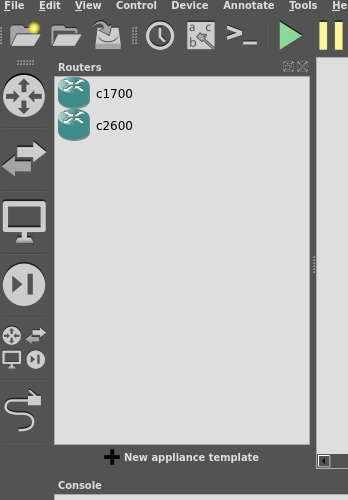
\includegraphics[width=10cm]{004.png}
\caption{Lista de roteadores configurados}
\label{Rotulo}
\end{figure}

\begin{figure}[H]
\centering
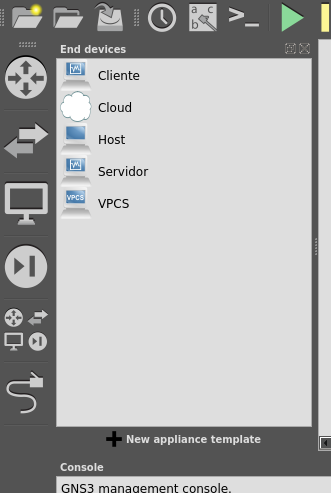
\includegraphics[width=10cm]{005.png}
\caption{Lista de hosts configurados}
\label{Rotulo}
\end{figure}

O roteador C1700 vem com duas interfaces disponíveis. Utilizaremos as seguintes WIC:

\begin{table}[H]
\centering
%\caption{Slots de interfaces do Roteador C1700}
\label{my-label}
\begin{tabular}{|l|l|}
\hline
WIC0 & WIC-1ENET \\ \hline
WIC1 & WIC-1ENET \\ \hline
\end{tabular}
\caption{Slots de interfaces do Roteador C1700}
\end{table}

\begin{figure}[H]
\centering
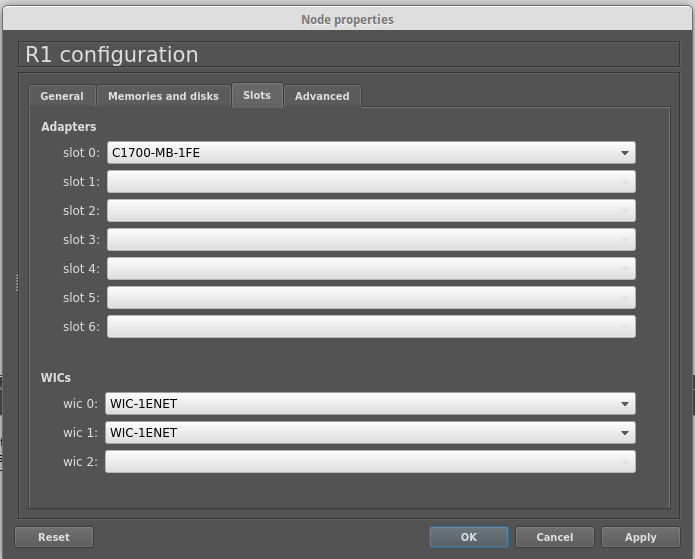
\includegraphics[width=10cm]{006.png}
\caption{Configuração de WICs do Roteador C1700}
\label{Rotulo}
\end{figure}


A interface WIC-1ENET fornecerá uma entrada Ethernet. Usaremos duas interfaces diferentes para obrigar o roteamento entre interfaces distintas.
% 1 entrada -> uma entrada
% sim, sou chato huahuahau

\subsection{Configuração da Topologia}

A nossa rede contará com um Roteador (C1700), dois switches e as nossas duas máquinas virtuais.
% 1 Roteador -> um roteador
% 2 switches -> dois switches
% eu pelo menos acho que fica melhor escrever os números por extenso, mas se vocês discordarem, dá pra deixar como tava

\begin{figure}[H]
\centering
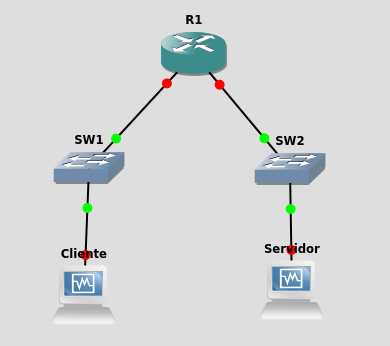
\includegraphics[width=10cm]{007.png}
\caption{Topologia utilizada para a Análise}
\label{Rotulo}
\end{figure}

Será utilizada esta topologia simples já que não possuímos um hardware potente o suficiente para simular redes maiores.
% hardware potente para simular -> hardware potente o suficiente para simular

\subsection{Configuração do Roteador Cisco C1700}

Com o roteador R1 - Cisco C1700 - iniciado, abriremos o seu console para aplicar as devidas configurações desejadas\cite{cisco-basic-commands} \cite{freeccnaworkbook}:

\begin{itemize}
  \item Uma única Rede 10.0.0.0/8 com duas subredes.
  \item Interface Ethernet0: 10.0.0.1 (Rede 10.0.0.0/16)
  \item Interface Ethernet1: 10.1.0.1 (Rede 10.1.0.0/16)
\end{itemize}

\begin{figure}[H]
\centering
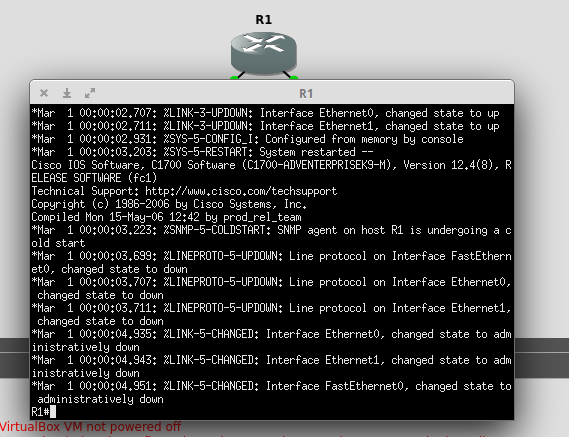
\includegraphics[width=12cm]{008.png}
\caption{Visão do Console do roteador Cisco C1700 no GNS3}
\label{Rotulo}
\end{figure}
% aumentei a largura de 10 pra 12 cm. Sei lá, parecia muito pequeno antes

\begin{lstlisting}[language=bash]
R1#configure terminal
Enter configuration commands, one per line. End with CNTL/Z.

R1(config)#interface Ethernet0
R1(config-if)#ip address 10.0.0.1 255.255.0.0
R1(config-if)#no shutdown
R1(config-if)#^Z
R1#show run interface Ethernet0

Building configuration...

Current configuration : 73 bytes
!
interface Ethernet0
 ip address 10.0.0.1 255.255.0.0
 half-duplex
end

\end{lstlisting}

\begin{lstlisting}[language=bash]
R1#configure terminal
Enter configuration commands, one per line. End with CNTL/Z.

R1(config)#interface Ethernet1
R1(config-if)#ip address 10.1.0.1 255.255.0.0
R1(config-if)#no shutdown
R1(config-if)#^Z
R1#show run interface Ethernet0

Building configuration...

Current configuration : 73 bytes
!
interface Ethernet0
 ip address 10.1.0.1 255.255.0.0
 half-duplex
end

\end{lstlisting}

\begin{table}[H]
\centering
%\caption{Tabela de interfaces no roteador R1}
\label{my-label}
\begin{tabular}{lll}
\hline
\multicolumn{1}{|l|}{Interface} & \multicolumn{1}{l|}{IP} & \multicolumn{1}{l|}{Mask} \\ \hline
Ethernet1                       & 10.1.0.0                & /16 255.255.0.0           \\
Ethernet0                       & 10.0.0.1                & /16 255.255.0.0          
\end{tabular}
\caption{Tabela de interfaces no roteador R1}
\end{table}

Como as duas redes estão ligadas diretamente ao roteador, não será necessário configurar a tabela de roteamento do roteador R1. A tabela poderá ser acessada da seguinte forma \cite{9tut} :

\begin{lstlisting}[language=bash]
R1#show ip route

Codes:  C- connected, S - static, R - RIP, M - mobile, B - BGP
        D - EIGRP, EX - EIGRP external, 0 - OSPF, IA - OSPF inter area
        N1 - OSPF external type 1, N2 - OSPF NSSA external type 2
        E1 - OSPF external type 1, E2 - OSPF external type 2
        i - IS-IS, su - IS-IS summary, L1 - IS-IS level-1, L2 - IS-IS level-2
        ia - IS-IS inter area, * - candidate default, U - per-user static route
        o - ODR, P - periodic downloades static route
   
Gateway of last resort is not set
    10.0.0.0/16 is subnetted, 2 subnets:
C   10.0.0.0 is directly connected, Ethernet0
C   10.1.0.0 is directly connected, Ethernet1

\end{lstlisting}

\begin{table}[H]
\centering
%\caption{Tabela de roteamento, roteador R1}
\label{my-label}
\begin{tabular}{llll}
\hline
\multicolumn{1}{|l|}{Tipo} & \multicolumn{1}{l|}{IP} & \multicolumn{1}{l|}{Máscara} & \multicolumn{1}{l|}{Próximo Passo} \\ \hline
C                          & 10.1.0.0                & 255.255.0.0                  & Ethernet1                          \\
C                          & 10.0.0.0                & 255.255.0.0                  & Ethernet0                         
\end{tabular}
\caption{Tabela de roteamento, roteador R1}
\end{table}

\section{Integração externa entre GNS3 e VirtualBox}

Para configurar os IPs \cite{howtoforge} das máquinas virtuais, será necessário acesso ao root e alteração dos devidos arquivos.

Alguns arquivos básicos de redes do Debian são:

\begin{itemize}  

    \item /etc/network/interfaces: Contém as configurações básicas das interfaces de rede. Pode-se configurar tanto IP quando Máscara da rede de forma estática ou por algum servidor DHCP.
    
    \item /etc/resolv.conf: Contém as configurações básicas de resolução. Pode-se configurar o servidor DNS.
    
    \item /etc/hosts: É o arquivo primário da resolução de nomes. Pode-se configurar IPs padrões para solucionar nomes. Em nosso teste, usaremos para acesso ao Servidor.

\end{itemize}

Após qualquer alteração é necessário reiniciar a interface de rede para realizar a releitura dos arquivos para a memória. Pode ser feita rapidamente utilizando o seguinte comando:

\begin{lstlisting}
service networking restart

# no Debian 7
# /etc/init.d/networking restart

# para verificar as configuracoes da rede
ifconfig
\end{lstlisting}

\subsection{Configuração dos IP's nas Máquinas Virtuais}

Para alterar o IP, realizamos a operação de Backup das configurações anteriores:

\begin{lstlisting}
mv /etc/network/interfaces /etc/network/interfaces.bak
\end{lstlisting}

Após isso, alteramos o arquivo /etc/network/interfaces original com a seguinte configuração:


\begin{lstlisting}[language=bash]
  auto lo
  iface lo inet loopback
  
  iface eth0 inet static
    address 10.1.0.20
    netmask 255.255.0.0
    network 10.1.0.0
    broadcast 10.1.255.255
    gateway 10.1.0.1
\end{lstlisting}

\begin{figure}[H]
\centering
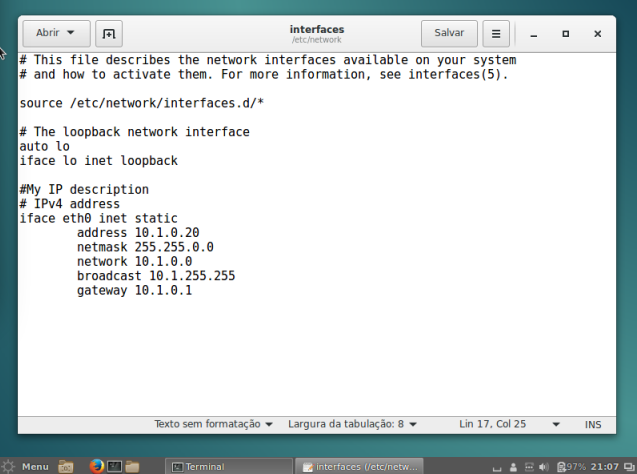
\includegraphics[width=12cm]{009.png}
\caption{Arquivo de configuração de redes no Debian}
\label{Rotulo}
\end{figure}
% de novo, 10 pra 12 cm


\begin{table}[H]
\centering
%\caption{Configuração de IPs das Máquinas Virtuais}
\label{my-label}
\begin{tabular}{|l|l|l|l|l|l|}
\hline
VM       & IP        & Máscara     & Network  & Broadcast    & Gateway  \\ \hline
Cliente  & 10.0.0.25 & 255.255.0.0 & 10.0.0.0 & 10.0.255.255 & 10.0.0.1 \\ \hline
Servidor & 10.1.0.1  & 255.255.0.0 & 10.1.0.0 & 10.1.255.255 & 10.1.0.1 \\ \hline
\end{tabular}
\caption{Configuração de IPs das Máquinas Virtuais}
\end{table}

\subsection{Configuração das Aplicações no Servidor}

Utilizaremos um servidor básico de HTTP para realizar os testes. A instalação dele é dada por este script:

\begin{lstlisting}[language=bash]
apt-get install apache2
apt-get install php5 php-pear php5-mysql
service apache2 restart
\end{lstlisting}

\section{Confirmação da Configuração}

\subsection{Traceroute}

Para confirmar se a nossa configuração está correta, utilizaremos a ferramenta Traceroute para Debian, a qual mostrará a rota entre o próprio \textit{Host} até outro \textit{Host}. Instalando em ambas as máquinas\cite{traceroute}:

\begin{lstlisting}[language=bash]
sudo apt-get install traceroute
\end{lstlisting}

\subsection{Resultado do Traceroute}

Executando o Traceroute, confirmamos o funcionamento da Topologia:

\begin{lstlisting}[language=bash]
# Executado no Cliente
traceroute 10.1.0.20
1 R1.eth1 10.1.0.1 320.320ms 320.119ms 332.241ms
2 Deb7Server 10.1.0.20 129.542ms 350.321ms 734.20ms
\end{lstlisting}

Ambas as máquinas virtuais estão configuradas corretamente, estabelecendo enlace entre as redes 10.1.0.0/16 e 10.0.0.0/16 separadas pelo roteador R1.